\documentclass[twoside,11pt]{article}
\usepackage{amsmath}
\usepackage{blindtext}
\usepackage{graphicx}
\usepackage{xcolor}
\usepackage{caption}
\usepackage{float}
% Any additional packages needed should be included after jmlr2e.
% Note that jmlr2e.sty includes epsfig, amssymb, natbib and graphicx,
% and defines many common macros, such as 'proof' and 'example'.
%
% It also sets the bibliographystyle to plainnat; for more information on
% natbib citation styles, see the natbib documentation, a copy of which
% is archived at http://www.jmlr.org/format/natbib.pdf

% Available options for package jmlr2e are:
%
%   - abbrvbib : use abbrvnat for the bibliography style
%   - nohyperref : do not load the hyperref package
%   - preprint : remove JMLR specific information from the template,
%         useful for example for posting to preprint servers.
%
% Example of using the package with custom options:
%
% \usepackage[abbrvbib, preprint]{jmlr2e}
\usepackage{jmlr2e}
\usepackage{url}
% Definitions of handy macros can go here

\newcommand{\dataset}{{\cal D}}
\newcommand{\fracpartial}[2]{\frac{\partial #1}{\partial  #2}}

% Heading arguments are {volume}{year}{pages}{date submitted}{date published}{paper id}{author-full-names}

\usepackage{lastpage}
% \jmlrheading{23}{2025}{1-\pageref{LastPage}}{1/21; Revised 6/25}{-/-}{21-0000}{Vishakh Begari}

% Short headings should be running head and authors last names

\ShortHeadings{Transformer Riffage}{Vishakh Begari}
\firstpageno{1}

\begin{document}
\title{Transformer Riffage}

\author{\name Vishakh Begari \email vibedjentle@gmail.com \\
       \addr Independent Researcher\\
       Bavaria, Germany\\
       ORCID: \href{https://orcid.org/0009-0008-9399-8581}{0009-0008-9399-8581}}

\editor{Adam Smasher}

\maketitle

\begin{abstract}%   <- trailing '%' for backward compatibility of .sty file
Ever since the electrification of guitar, there has been an explosion 
in rhythmic complexity, tone experimentation and playing techniques. Music 
generation using Transformers \cite{Vaswani2} has generally 
been used for creating mostly musical notes. In this paper, a new approach is proposed 
to capture the diverse expressions commonly featured in modern metal music. 
A new tokenisation method encapsulates the various guitar techniques and a sequence level attention component 
which tries to capture the segmentation between different musical phrases.
An inference method is implemented that provides meaningful validation without human evaluation.
\end{abstract}

\begin{keywords}
  Transformer models, Music, Generative, Sequence modelling, Attention mechanism
\end{keywords}

\section{Introduction}
A \textit{riff} is a short, repeated motif or figure in the melody or accompaniment of a 
musical composition. \cite{randel:86} This type of composition is particularly prevalent 
in rock, metal, blues, funk and jazz. It is often the main feature that gives character 
and structure to a song. Recent developments in Transformers architecture have inspired 
many to generate sequences by treating musical notes as symbolic language. 

Musical elements like notes, timestamps, and velocities are converted into discrete tokens similar to 
text processing. \cite{aws_deepcomposer} A widely adopted method for representing musical notes digitally is the MIDI format, 
which encodes pitch, duration, and dynamics. Using such a format for musical expression has limitations like resolution 
and bandwidth constraints \cite{midi_short} when compared to richer representations like 
audio recordings and detailed scores. Modern guitar riffs frequently employ intense and abrupt expressive
techniques, which contribute significantly to its overall identity. To accurately represent the nuanced 
expressive elements of modern music, a score-based format is preferable over simpler encodings like MIDI.
A comprehensive list of these expressive elements is provided in Appendix~\ref{app:A}. Generating modern music 
demands capturing not only note patterns but also the associated expressions. 

\section{Encoding}
The original Transformer model \cite{Vaswani} used a vocabulary of tokens derived from the input language corpus, with each token 
represented as an integer index. A note is represented by multiplying the guitar’s fret number by the string number to 
generate a unique index. This approach not only helps the model learn the patterns of movement on the fretboard 
but also provides flexibility to accommodate alternative tunings, which are increasingly common in modern guitar playing.
With 6 strings and 23 frets per string, the instrument offers 138 distinct fretboard positions. The rhythmic structure is 
divided into seven beat durations: whole, 1/2, 1/4, 1/8, 1/16, and 1/32 and 1/64 notes. 
These divisions provide varying levels of temporal granularity for representing note durations. Each beat can further be 
subdivided into 14 distinct rhythmic values which is listed in Appendix~\ref{app:C}, which makes a total to 82 unique beat indices.
Since palm muting is a prominent feature in metal music, 
it is assigned a unique token in the representation. This encoding process produces 138 * 98 * 2 = 27048 unique musical tokens. 
The expressive vocabulary listed in Appendix~\ref{app:A} is represented using the same format. A unique integer is assigned to various accents used in guitar playing.
The necessity of using relative positional encodings rather than absolute ones, is already shown to enable state reuse without causing temporal confusion \cite{XL}. 
Since music is highly sequential such an encoding type should preserve timing, order, and spacing between notes.

Let \( L \) be the sequence length and \( d \) be the dimensionality of each attention head.

We define the relative positional embedding matrix:
\[
\mathbf{R} \in \mathbb{R}^{(2L - 1) \times d}
\]
where the size \(2L - 1\) corresponds to all possible relative positions from \(- (L - 1)\) to \(+(L - 1)\).

The embedding lookup for a relative position \(r = j - i\) (shifted by \(L - 1\) to be non-negative) is given by:
\[
\mathbf{r}(r) = \mathbf{R}[r + (L - 1)], \quad r \in \{-(L-1), \ldots, 0, \ldots, (L-1)\}
\]

Here, \(\mathbf{r}(r) \in \mathbb{R}^d\) is the embedding vector corresponding to relative position \(r\).


\subsection{Note representations}
\label{sec:note-representations}
The formula for note encodings is given by: 
\begin{align}
note\_encodings = ni + bt * 276 + bb * 276 * 14
\end{align}
\begin{align}
ni = fn + sn * 23 + 6 * 23 * nval
\end{align}
\begin{align}
nval =
\begin{cases}
1& \text{if, Palm Mute} \\
0 & \text{otherwise} \\
\end{cases}
\end{align}
\begin{align}
bt =
\begin{cases}
1 + d & \text{if, Triplet(3)} \\
2 + d & \text{if, Quintuplet(5)} \\
3 + d & \text{if, Sextuplet(6)} \\
4 + d & \text{if, Septuplet(7)} \\
5 + d & \text{if, Nonuplet(9)} \\
6 + d & \text{if, Undecuplet(11)}\\
\end{cases}
\end{align}
\begin{align}
d =
\begin{cases}
7& \text{if, Dotted note} \\
0 & \text{otherwise} \\
\end{cases}
\end{align}
\begin{align}
bb =
\begin{cases}
0 & \text{if, 1 / 64} \\
1 & \text{if, 1 / 32} \\
2 & \text{if, 1 / 16} \\
3 & \text{if, 1 / 8} \\
4 & \text{if, 1 / 4} \\
5 & \text{if, 1 / 2} \\
6 & \text{if, 1 / 1} \\
\end{cases}
\end{align}

\subsection{Accent representations}

\subsubsection{chord}
A chord is a group of notes played together, typically three or more. Figure~\ref{fig:accent} depicts a C major chord comprising of 3 notes - root note [C] played on the fret 2 / 5th string , major third [G] on fret 1 / 4th string and perfect fifth [E] on fret 2 / 1st string. 

\begin{figure}[htbp]
  \centering
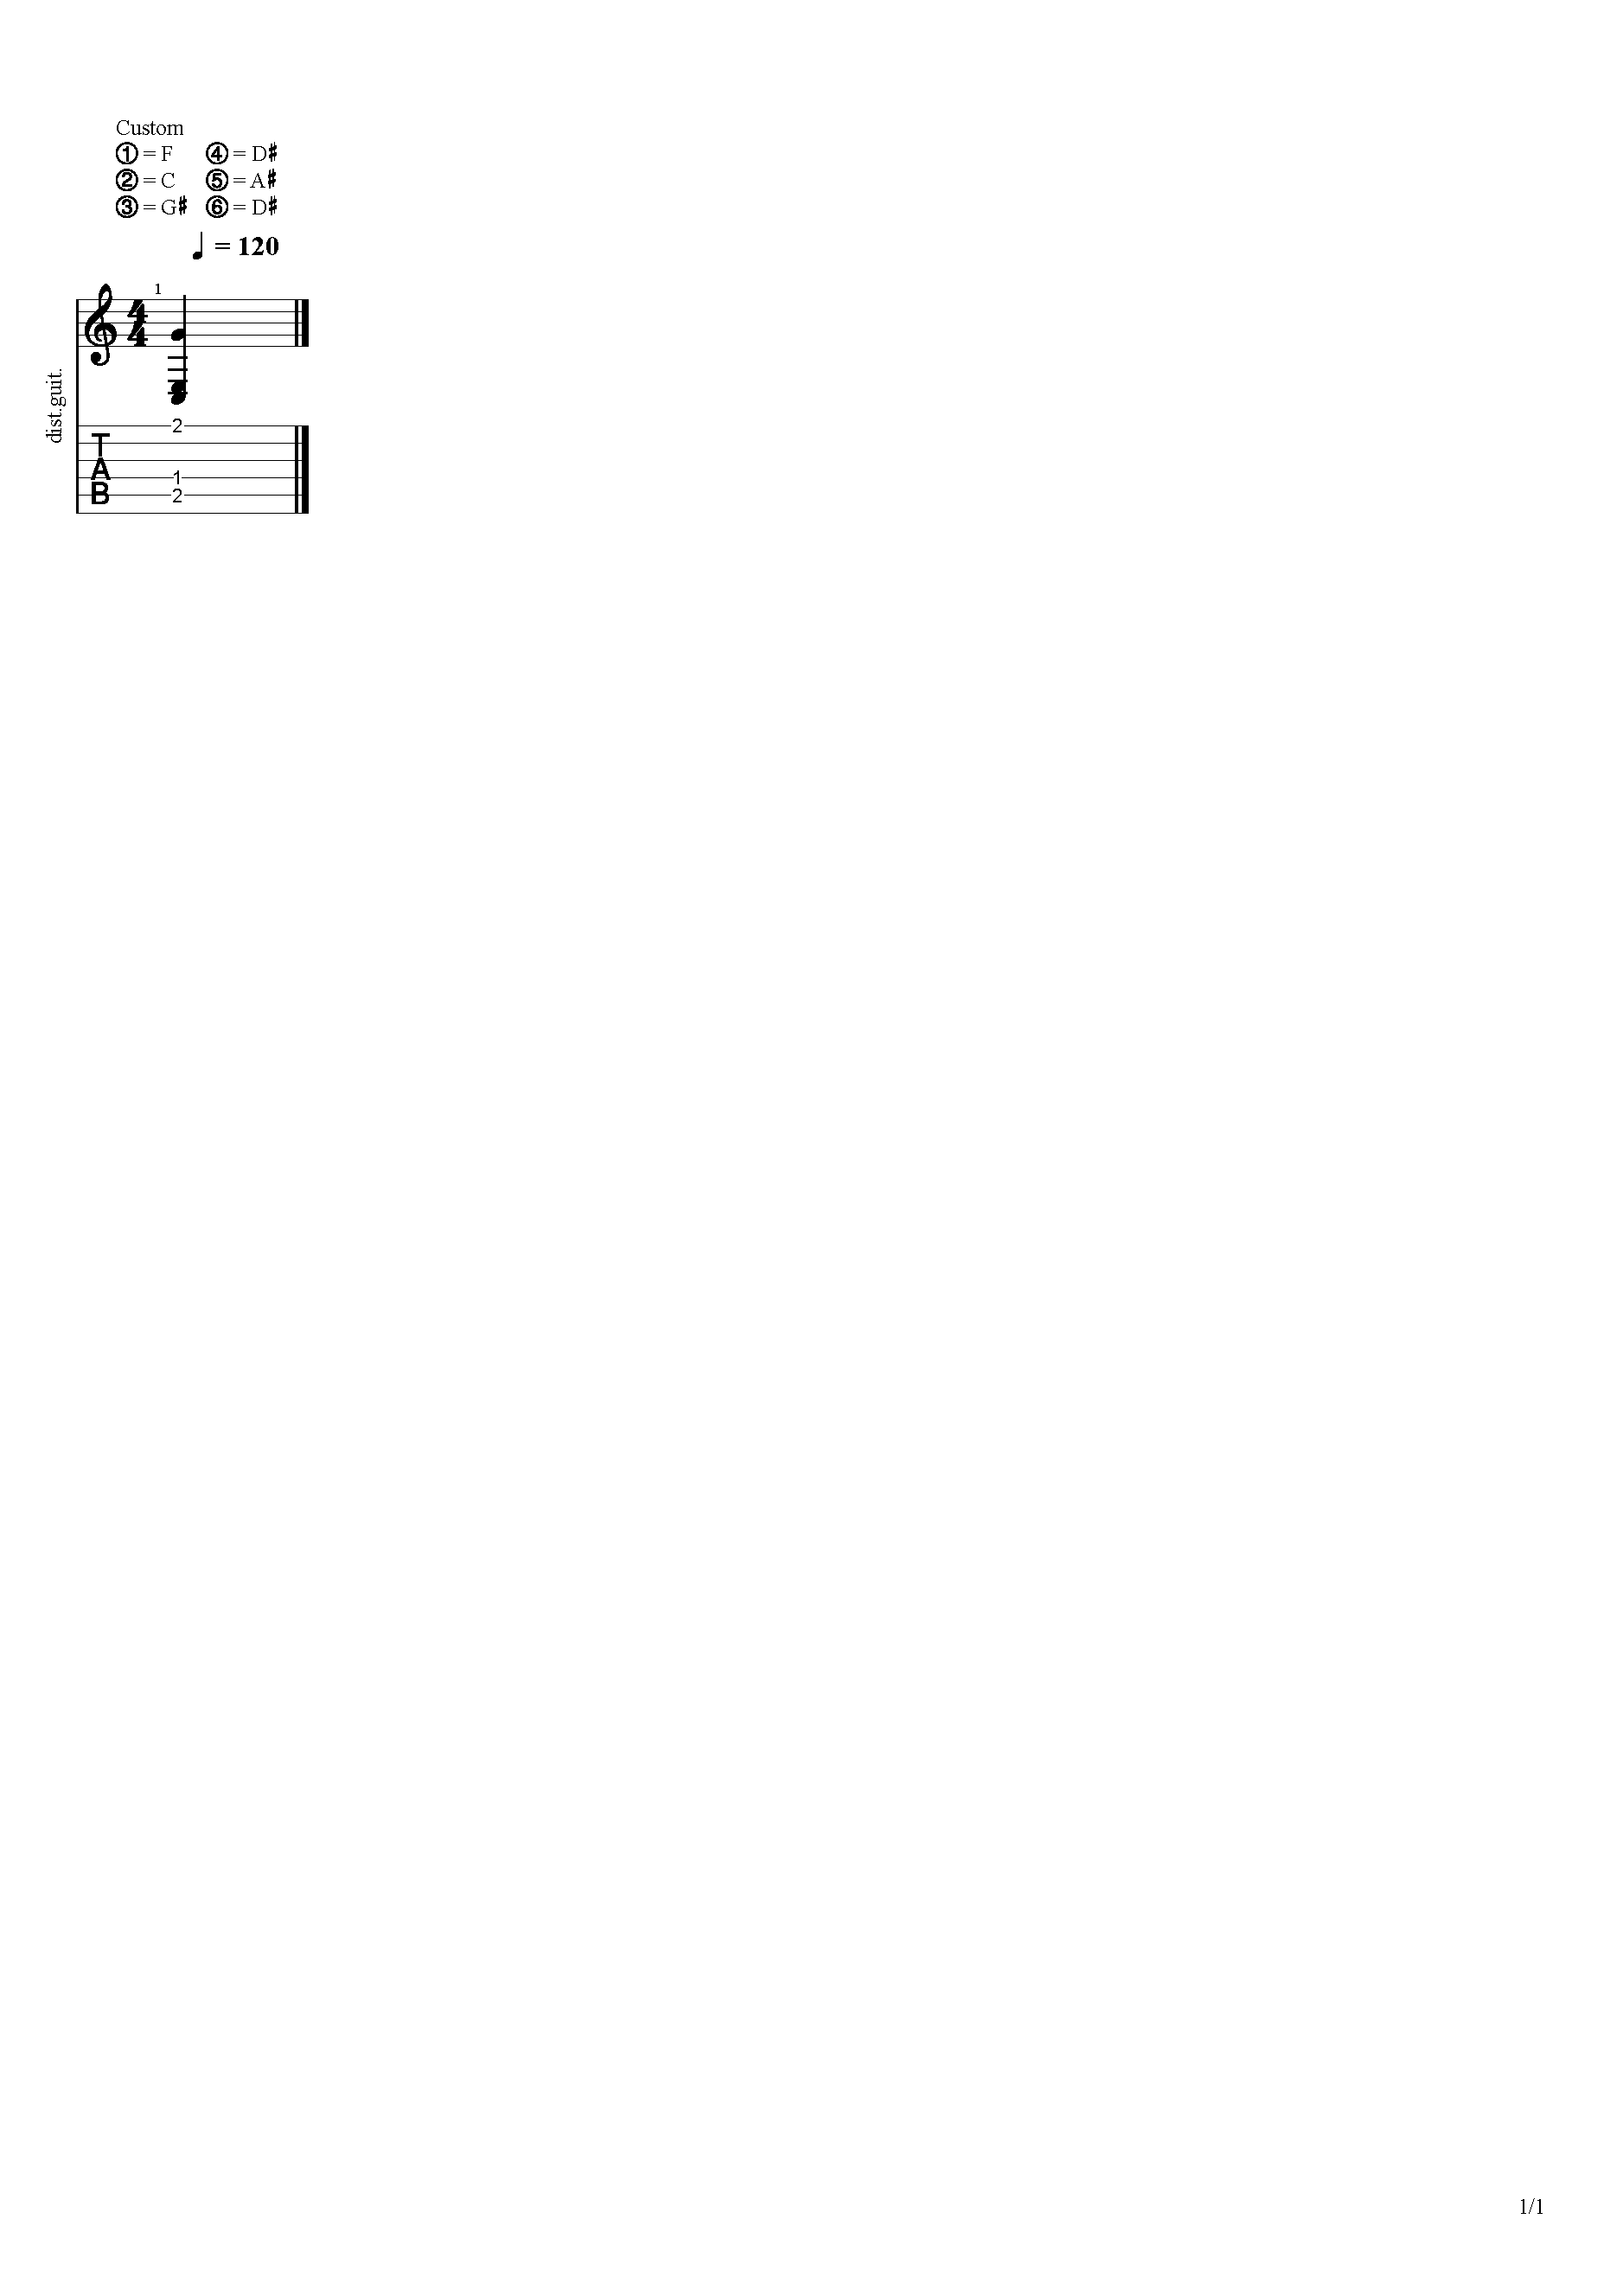
\includegraphics[trim={0 1120 710 60}, clip, width=0.3\linewidth]{Cmajor.pdf}
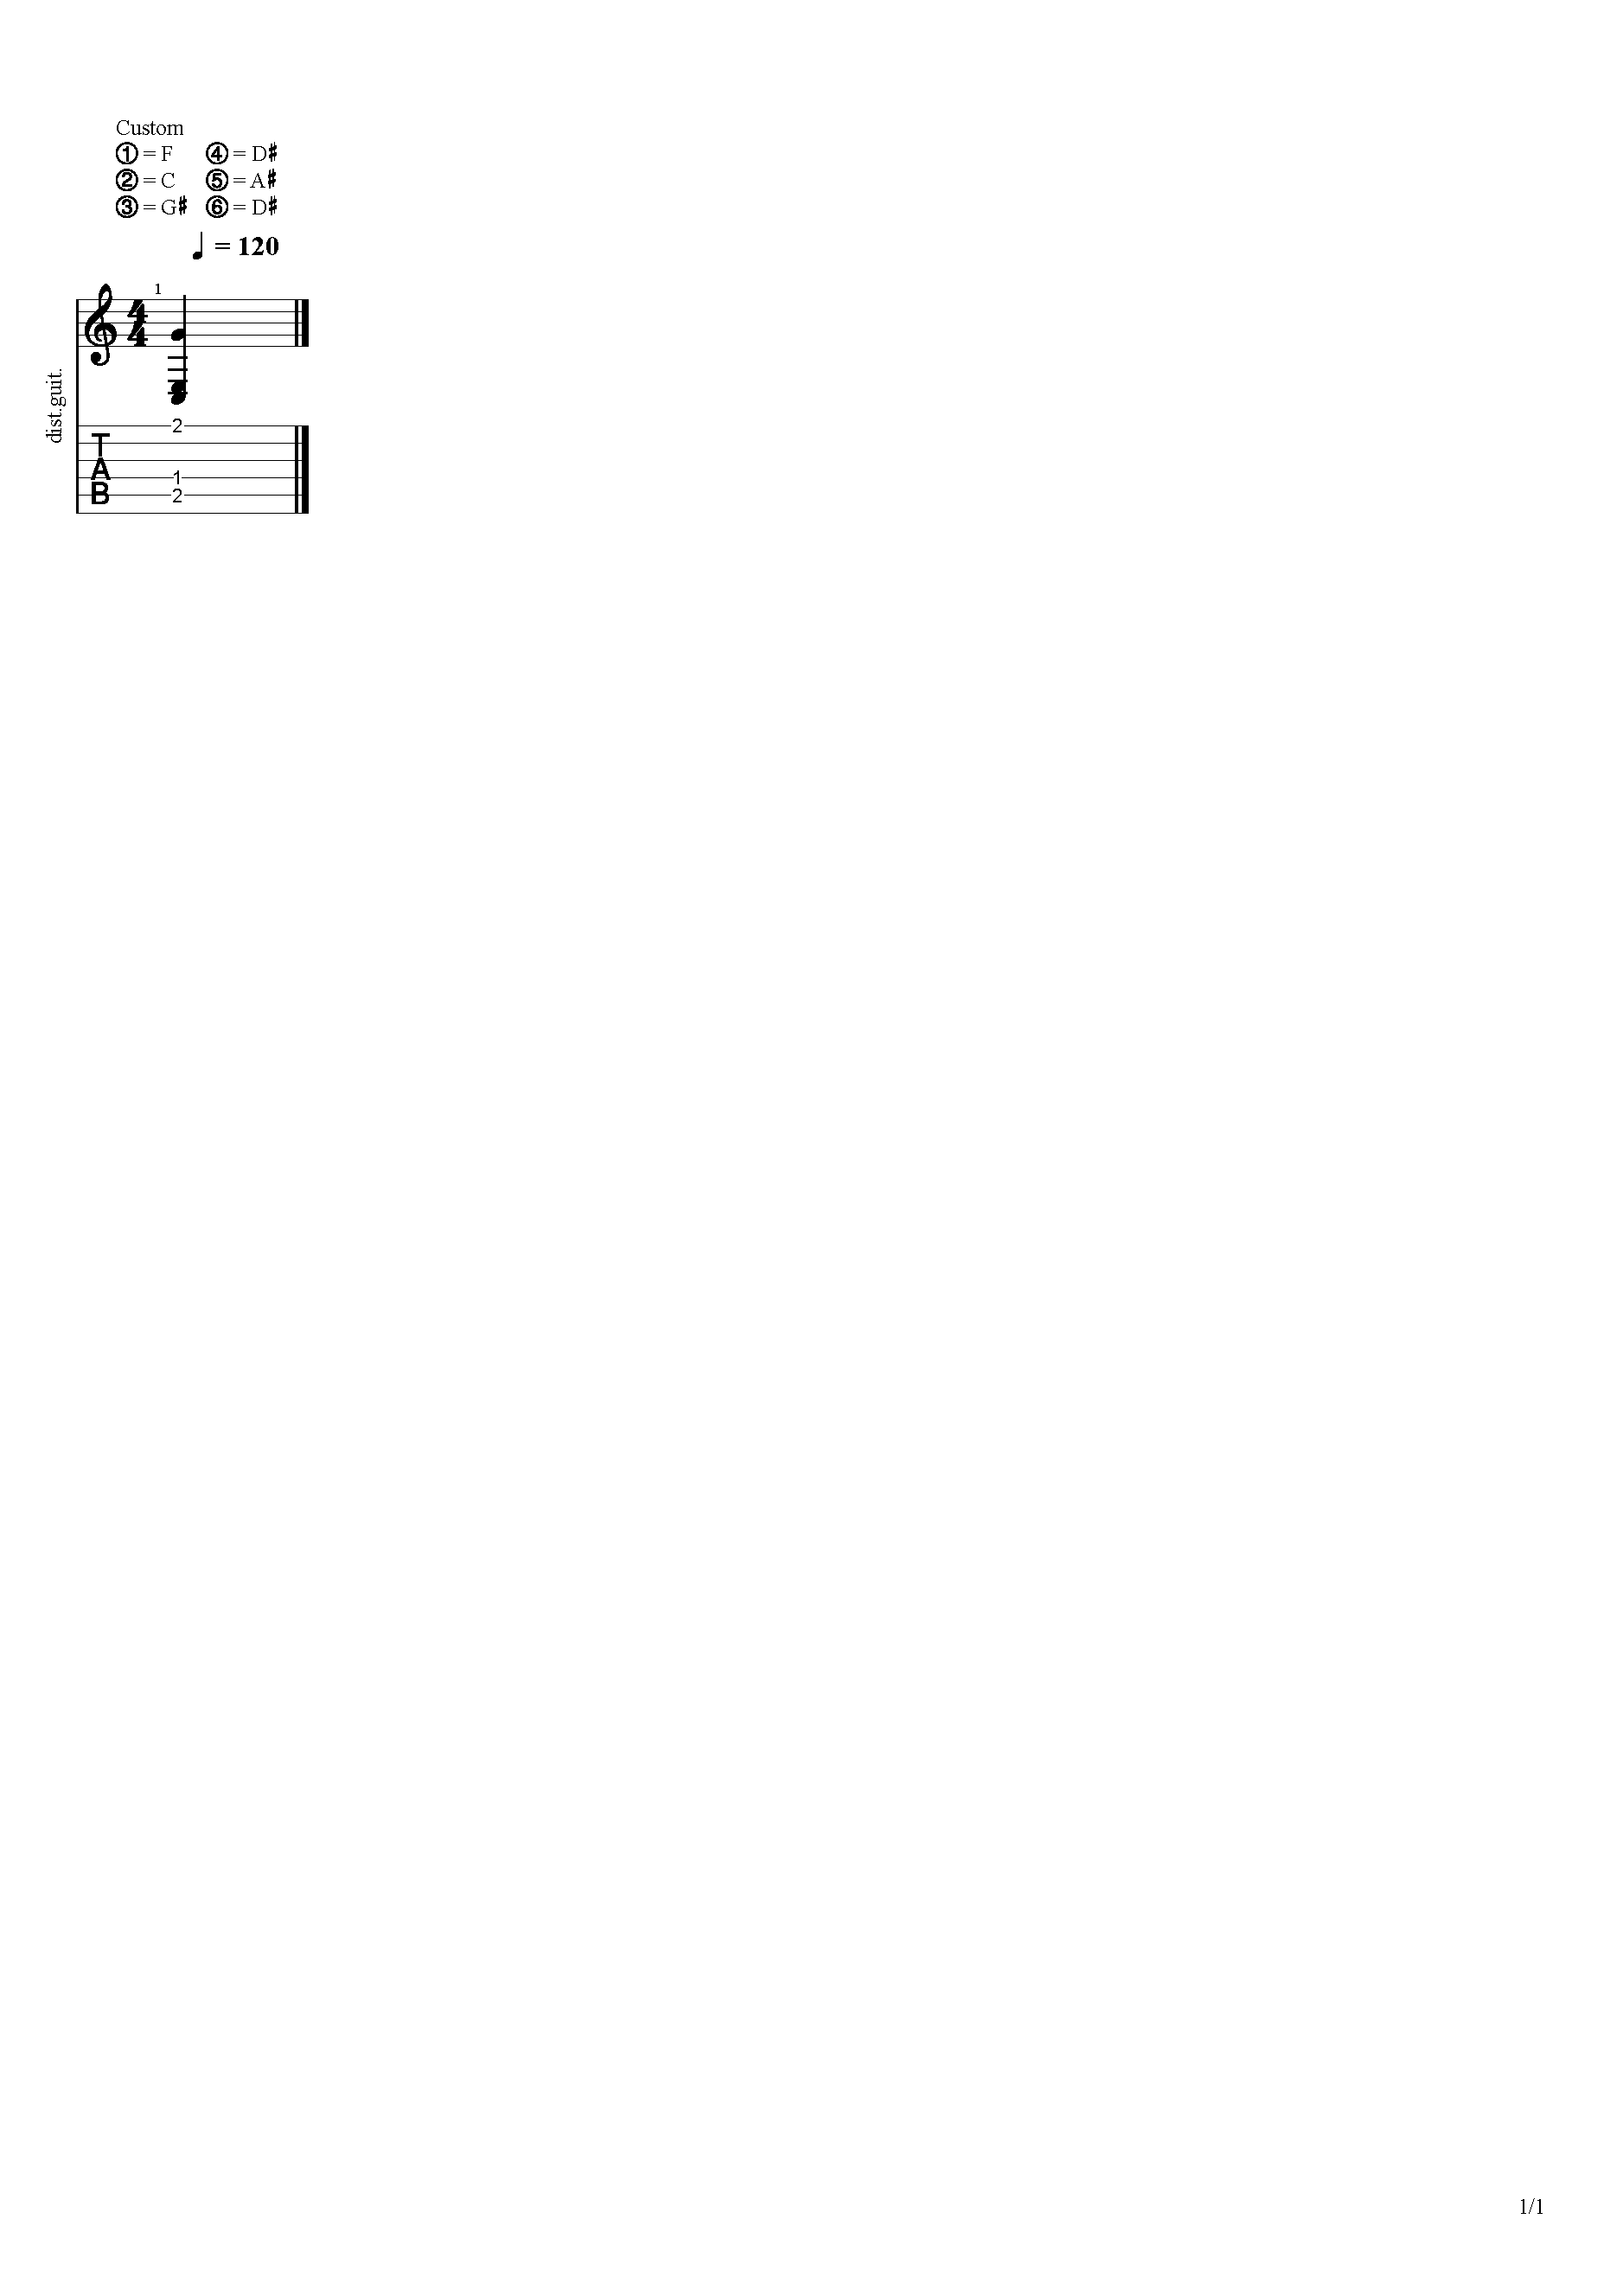
\includegraphics[trim={0 980 650 150}, clip, width=0.4\linewidth]{Cmajor.pdf}
\caption{C major chord shape on a 6 string with custom tuning.}
  \label{fig:accent}
\end{figure}

\begin{table}[h!]
\begin{center}
\begin{tabular}{cccccc}
  \hline
  \multicolumn{1}{|c|}{15413} & \multicolumn{1}{|c|}{27051} & \multicolumn{1}{|c|}{15389} & \multicolumn{1}{|c|}{27051} & \multicolumn{1}{|c|}{15321} & \multicolumn{1}{|c|}{27051} \\
   \hline
  \textcolor{gray}{C} & \textcolor{gray}{BARRE\_NOTE}  & \textcolor{gray}{E}   & \textcolor{gray}{BARRE\_NOTE}  & \textcolor{gray}{G} & \textcolor{gray}{BARRE\_NOTE} \\
\end{tabular}
\end{center}
\caption{C major chord quarter note tokenisation in a sequence.}
\label{tab:chordindexing}
\end{table}

\subsubsection{other}
Accentuations like BEND\_NOTE, SLIDE\_NOTE etc are represented by the note encodings from Section~\ref{sec:note-representations} followed by an accent token listed in Appendix~\ref{app:A}.
\begin{figure}[htbp]
  \centering
  \begin{minipage}[b]{0.48\linewidth}
    \centering
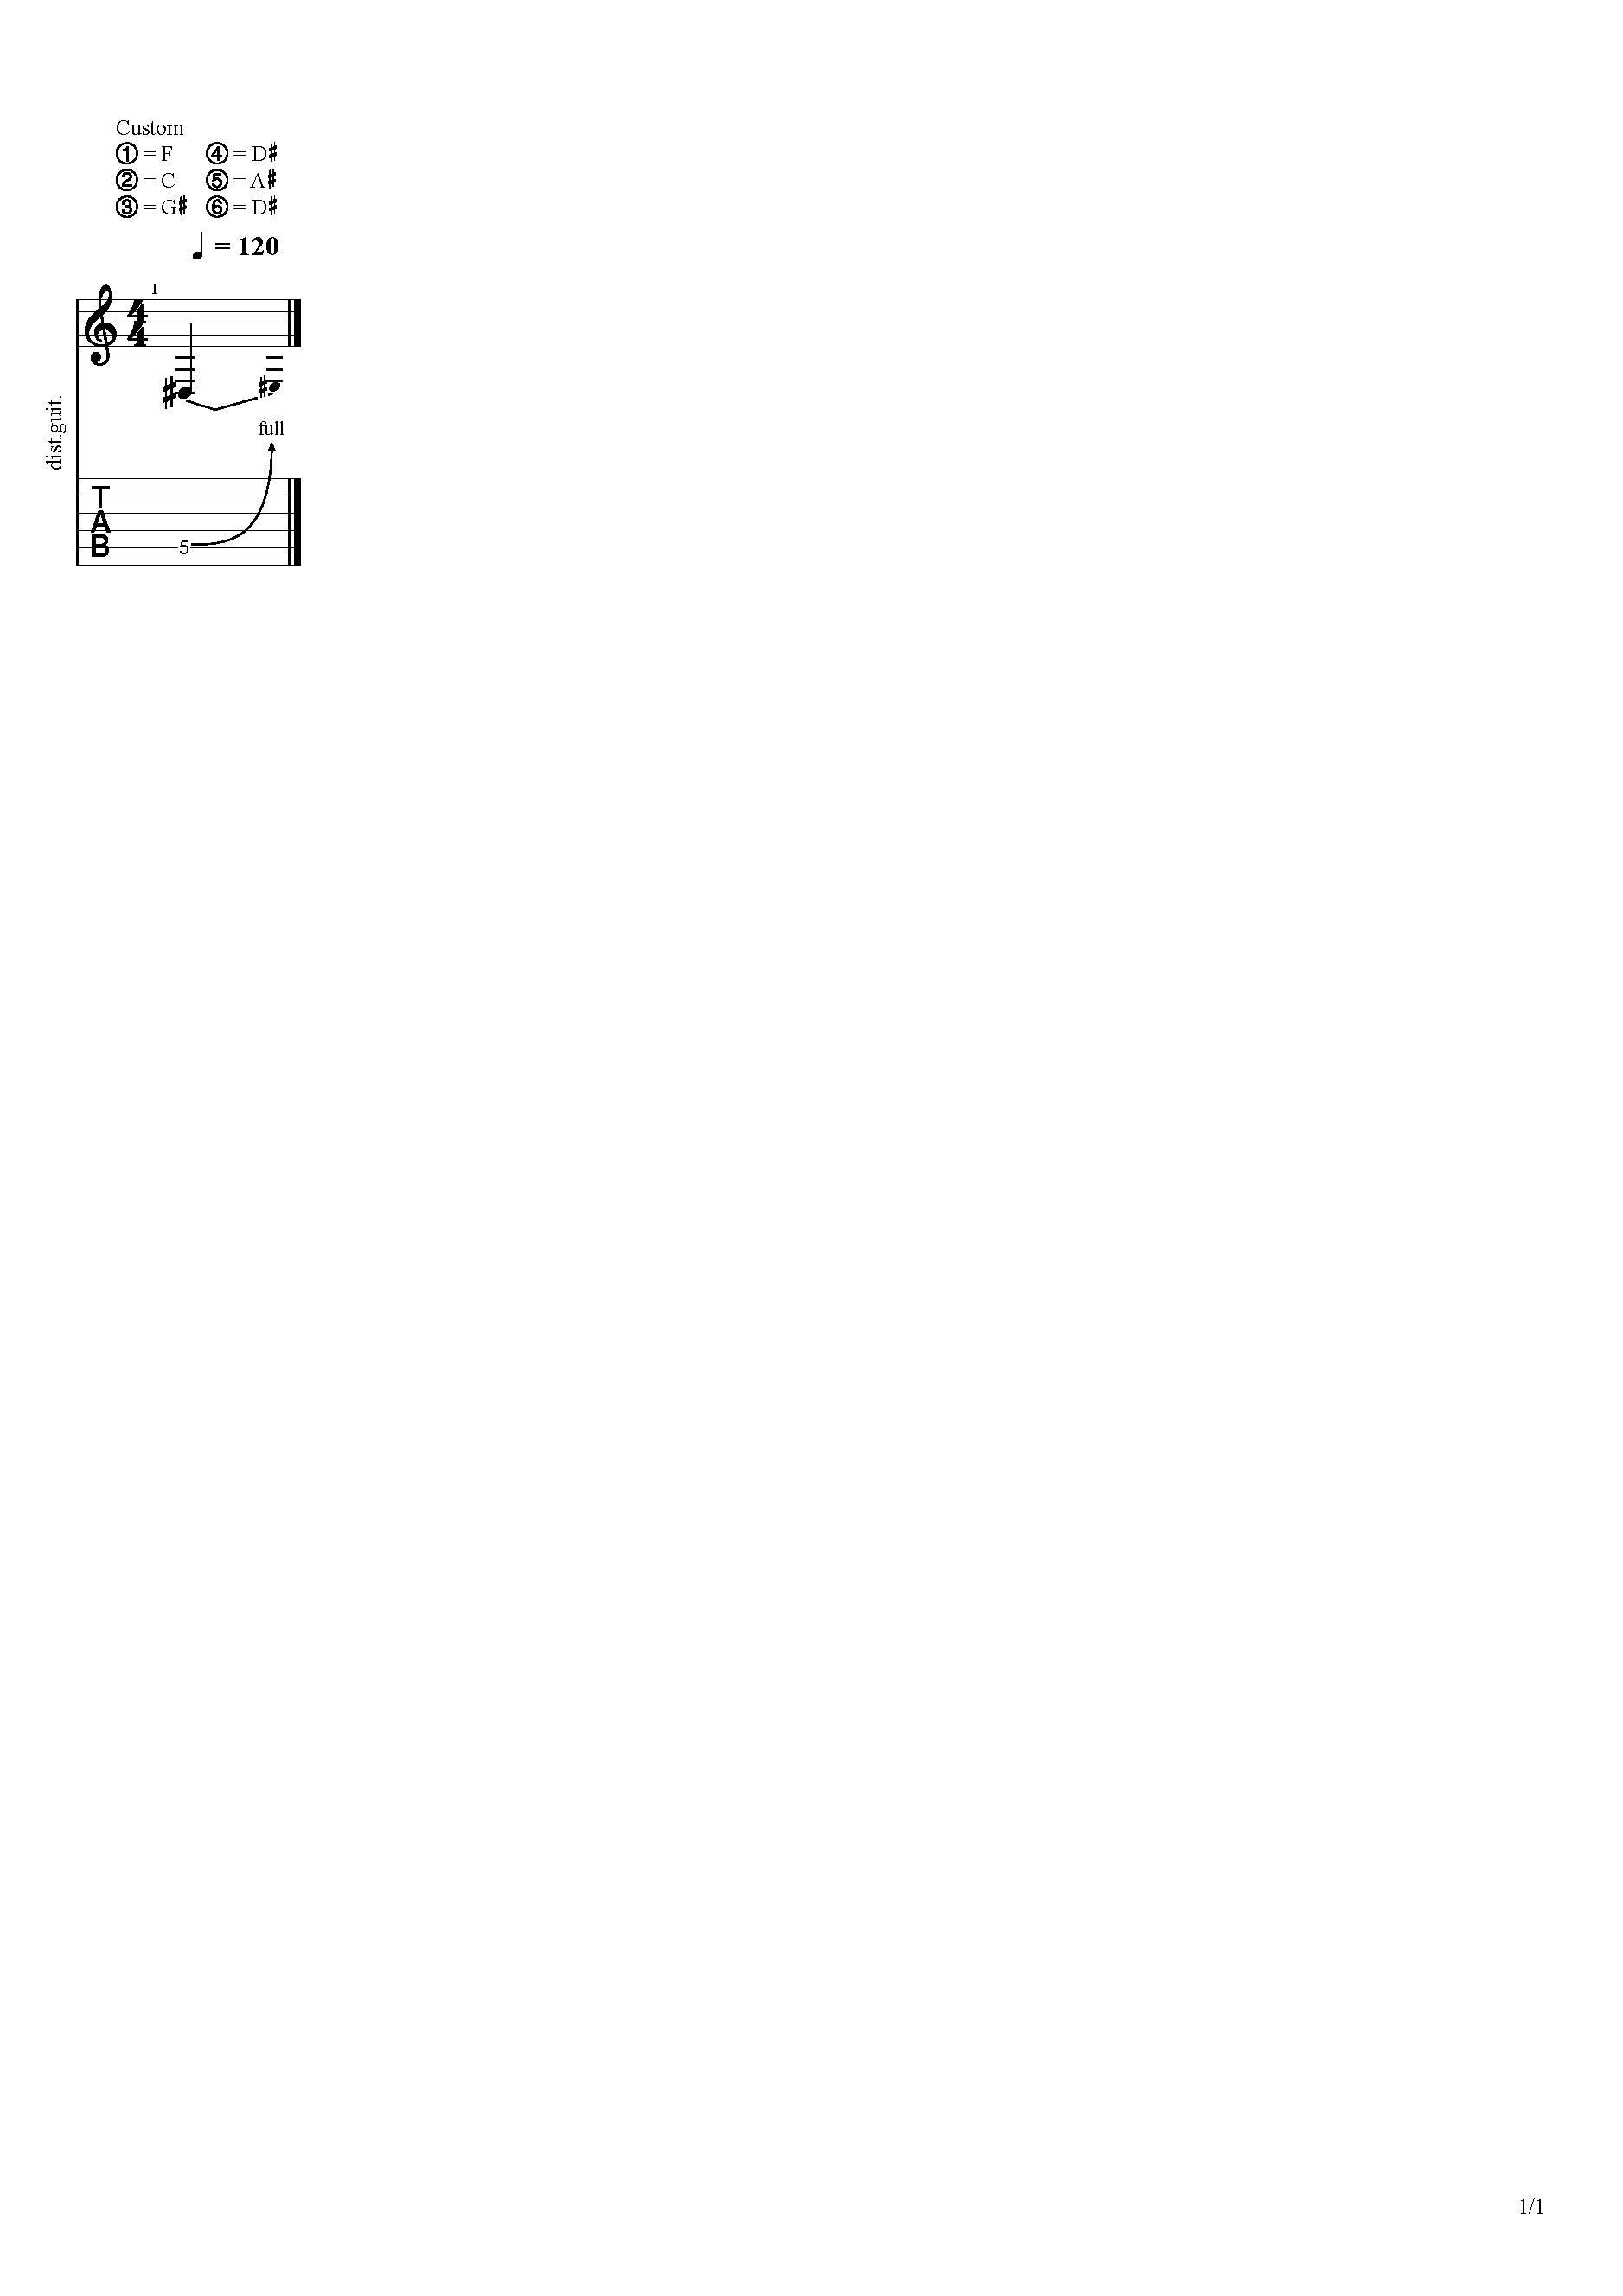
\includegraphics[trim={0 950 650 130}, clip, width=0.6\linewidth]{Note5bend1.pdf}
\captionsetup{type=figure}
\caption{Fret 5 string 5 quarter note bend}
  \label{fig:bend}
\end{minipage}
  \hfill
\begin{minipage}[b]{0.40\linewidth}
\centering
\begin{tabular}{cc}
  \hline
  \multicolumn{1}{|c|}{15416} & \multicolumn{1}{|c|}{27052}\\
   \hline
  \textcolor{gray}{C} & \textcolor{gray}{BEND\_NOTE\_1}
\end{tabular}
\captionsetup{type=table}
\caption{Bend note tokenisation}
\label{tab:bendindexing}
\end{minipage}
\end{figure}

\subsection{EOS and BAR}
A music bar (also called a measure) is a fundamental unit in musical notation that divides music into segments of equal time, defined by the time signature. Each bar is separated by a BAR token.
A collection of measures making a song is separated by an EOS token.

\section{Embedding}
A bar consists of a fixed number of beats, composed of musical notes that were tokenised as described in the previous section. Each bar is treated like a sentence.
The tokens representing the accents or expression in riff are placed next to each note in the sentence. An example of 
a riff and its tokenisation is given in Figure~\ref{fig:bend} . It has been demonstrated that the transformer equipped with relative attention is very well-suited for generative modelling of symbolic music. \cite{Vaswani2}. The chunking strategy used to carry over context between sequences during training follows the approach introduced in \cite{chunking}, which builds upon Transformer-XL’s segment-level recurrence mechanism. This method enables the model to capture longer-range dependencies by reusing hidden states from previous token chunks across segments.

\section{Training}
\subsection{Model}
The Transformer is built from a decoder-only stack with masked self attention as described in \cite{Vaswani2}. Although, segment-level recurrence mechanism is captured in Transformer-XL \cite{transformerXL},  its memory is limited to one previous segment at a time. To model dependencies across a whole batch, the gaussian distributions of the sequences are learned through a Multi layer Perceptron layer.
If the input is a batch of sequences defined by:
\begin{align}
X \in \mathbb{R}^{B \times T \times d}
\end{align}
Where:
\begin{itemize}
    \item \( B \): batch size (number of sequences)
    \item \( T \): number of tokens per sequence
    \item \( d \): embedding dimension
    \item \( X_i \in \mathbb{R}^{T \times d} \): the \(i\)-th sequence in the batch
\end{itemize}

Sequence level mean pooling is performed by:
\begin{align}
\bar{x}_i = \frac{1}{T} \sum_{t=1}^{T} X_{i,t} \quad \in \mathbb{R}^{d}
\end{align}

Gaussian parameters are then computed with a Multi Layer Perceptron.
Let \( f: \mathbb{R}^{d} \rightarrow \mathbb{R}^{2d} \) be a learned MLP.
Then:
\begin{align}
[\mu_i, \log \sigma_i] = f(\bar{x}_i)
\quad \text{with} \quad 
\mu_i, \log \sigma_i \in \mathbb{R}^{d}
\end{align}

Ensure positivity of standard deviation:
\begin{align}
\sigma_i = \exp(\log \sigma_i) + \varepsilon
\quad \text{where } \varepsilon > 0
\end{align}

Each sequence is then represented as a diagonal multivariate Gaussian:
\begin{align}
\mathcal{N}_i = \mathcal{N}(\mu_i, \mathrm{diag}(\sigma_i^2))
\end{align}

Vectorized for the batch:
\begin{align}
[\mu, \log \sigma] = f(\bar{X}) \in \mathbb{R}^{B \times 2d}
\end{align}
\begin{align}
\sigma = \exp(\log \sigma) + \varepsilon \in \mathbb{R}^{B \times d}
\end{align}

The pairwise KL divergence between each pair of Gaussians \cite{kldiv}:
\begin{align}
\label{eq:kldiv}
\text{KL}(\mathcal{N}_i \parallel \mathcal{N}_j) =
\frac{1}{2} \sum_{k=1}^{d} \left[
\log\left( \frac{\sigma_{j,k}^2}{\sigma_{i,k}^2} \right) +
\frac{\sigma_{i,k}^2}{\sigma_{j,k}^2} +
\frac{(\mu_{i,k} - \mu_{j,k})^2}{\sigma_{j,k}^2} - 1
\right]
\end{align}

This produces a KL matrix:
\begin{align}
\text{KL\_matrix} \in \mathbb{R}^{B \times B}, \quad
[\text{KL\_matrix}]_{i,j} = \text{KL}(\mathcal{N}_i \parallel \mathcal{N}_j)
\end{align}

A simpler version of the attention matrix from \cite{XL} is used from which the KL divergence-based sequence bias is subtracted:
\begin{align}
\text{RA}_{\text{KL}} = \text{softmax} \left( \frac{Q K^\top}{\sqrt{d_k}} + Q R^\top - \alpha \cdot \text{KL}_{\text{bias}} \right)
\end{align}
A weighted sum over relative positional value contributions $V_{\text{rel}}$ is then added:
\begin{align}
\text{Output} = \text{RA}_{\text{KL}} \times V + \text{RA}_{\text{KL}} \times V_{\text{rel}}
\end{align}
\subsection{Loss function}
The model's loss is composed of three components:
\begin{align}
Totalloss=CrossEntropy + Repetition loss + Sequence loss
\end{align}
\subsubsection{Cross Entropy loss}
Cross-entropy loss is the standard choice for training deep neural networks and logistic regression models for both binary and multi-class classification tasks. \cite{mlglossary}
\subsubsection{Repetition loss}
Repetition helps organise musical ideas, making pieces more 
coherent and memorable. It gives listeners reference points and expectations, 
aiding in the recognition and recall of themes or motifs. \cite{Hu_2022}
Composers have long used stochastic (probability-based) methods to inject randomness into repeated motifs, 
sometimes even employing quantum randomness for truly unpredictable results. \cite{yamada_grandi_munoz-gil_barbiero_aloy_lewenstein_2021} This demands careful consideration, as it relies on the listener’s inherent ability to recognise patterns and their natural inclination toward novelty. 
Since it is already known that tokens listed in Appendix A cannot repeat, it is penalised through repetition loss making them less likely to be selected again in subsequent steps. 
A variant of the repetition penalty introduced in \cite{reppenalty} is employed; however, instead of greedy decoding, multinomial sampling is used to generate tokens to get semantically different output sequences \cite{song2024}. Including this loss during training eliminates the need to explicitly handle constraints for generating valid sequences at inference time
\begin{align}
\text{Let } p_{b,t,v} = \text{softmax}\left( \frac{\text{logits}_{b,t,v}}{T} \right), \quad \text{for } b = 1,\dots,B;\ t = 0,\dots,T-1;\ v = 1,\dots,V \\[1ex]
\end{align}
Compute average past probabilities:
\begin{align}
\bar{p}_{b,t,v} = \frac{1}{t} \sum_{k=0}^{t-1} p_{b,k,v}, \quad \text{for } t \geq 1
\end{align}
Repetition score (dot product of current and average previous probabilities)
\begin{align}
R_{b,t} = \sum_{v=1}^{V} p_{b,t,v} \cdot \bar{p}_{b,t,v}, \quad \text{for } t \geq 1
\end{align}
Final penalty (mean repetition score across batch and sequence, excluding)
\begin{align}
\qquad Repetition loss = \frac{\lambda}{B(T - 1)} \sum_{b=1}^{B} \sum_{t=1}^{T-1} R_{b,t}
\end{align}
where $\lambda$ is a repetition penalty weight hyper parameter.

\subsubsection{Sequence Penalty loss}
Pairwise KL divergence between each pair of Gaussians is given by~\eqref{eq:kldiv}. 
Given a batch of \( B \) sequences, Sequence loss is defined by:

\begin{align}
\mathcal{L}_{\text{KL}} = \frac{1}{B} \sum_{b=1}^B \text{KL}(\mathcal{N}_q^{(b)} \,\|\, \mathcal{N}_k^{(b)})
\end{align}
To make the training more stable, the sequence loss is annealed and clamped. 
\begin{align}
Sequenceloss = \min\left( \frac{\text{step}}{\text{EPOCHS}} \cdot \left( \frac{\delta \cdot \mathcal{L}_{\text{KL}}}{\text{BATCH}} \right),\ 0.2 \right)
\end{align}
where, $\delta$ is a sequence weight hyper parameter.
\subsubsection{Dataset}
Relavant statistics about the dataset used for training and evaluation are provided in Appendix~\eqref{app:B}
\begin{figure}[H]
  \centering

\includegraphics[clip, width=0.7\linewidth]{trainingaccentprobability.pdf}
\caption{Accent occurrences in training data for a random seed.}
  \label{fig:accentnote}
\end{figure}
\begin{figure}[H]
  \centering

\includegraphics[clip, width=0.7\linewidth]{startprobability.pdf}
\caption{Token occurrences of first note of a musical measure in training data.}
  \label{fig:firstnote}
\end{figure}
\subsection{Grid search over Hyper-Parameters}
To determine the optimal configuration, a grid search was performed over a predefined set of hyperparameter values. 
The search included combinations of key parameters such as learning rate, sequence length, model dimensionality, 
Each configuration was trained for 10 epochs, and performance was evaluated on a validation set using loss. 
The best-performing set of hyperparameters was selected based on the lowest validation score.

\section{Inference}
Given that the model is autoregressive and expects an initial token, selecting the start token based on the 
distribution of starting notes of musical measures in the training data yields more consistent generation.

The idea of context carryover has been well-established in \cite{context}. During inference, the model carries over context from previous sequences by using the last token of the preceding measure as the first token for the subsequent measure.
To compare the quality of predicted tokens (P)  from true distributions (Q), relative entropy is calculated using Kullback-Leibler divergence:
\begin{align}
D_{\mathrm{KL}}(P \parallel Q) = \sum_{x \in X} P(x) \log \left( \frac{P(x)}{Q(x)} \right)
\end{align}

The reported loss values were computed as the mean over five independent training runs after 100 epochs for hyper-parameter values listed in Appendix~\eqref{app:D}:
\begin{table}[H]
 \centering
\begin{tabular}{ccc}
\hline
  \multicolumn{1}{|c|}{\textbf{Loss}} & \multicolumn{1}{|c|}{\textbf{Mean}} & \multicolumn{1}{|c|}{\textbf{Std. dev.}}\\
  \hline
  \multicolumn{1}{|c|}{Cross Entropy} & \multicolumn{1}{|c|}{1.6827} & \multicolumn{1}{|c|}{0.0437}\\
  \hline
  \multicolumn{1}{|c|}{Repetition} & \multicolumn{1}{|c|}{0.0323} & \multicolumn{1}{|c|}{0.0002}\\
  \hline
  \multicolumn{1}{|c|}{Sequence} & \multicolumn{1}{|c|}{0.1996} & \multicolumn{1}{|c|}{1e-6}\\
  \hline
  \multicolumn{1}{|c|}{Total} & \multicolumn{1}{|c|}{1.8021} & \multicolumn{1}{|c|}{0.1051}\\
  \hline
  \multicolumn{1}{|c|}{Validation} & \multicolumn{1}{|c|}{1.8021} & \multicolumn{1}{|c|}{0.1051}\\
    \hline
\end{tabular}
\captionsetup{type=table}
\caption{Loss values}
\label{tab:loss}
\end{table}

\begin{figure}[H]
  \centering
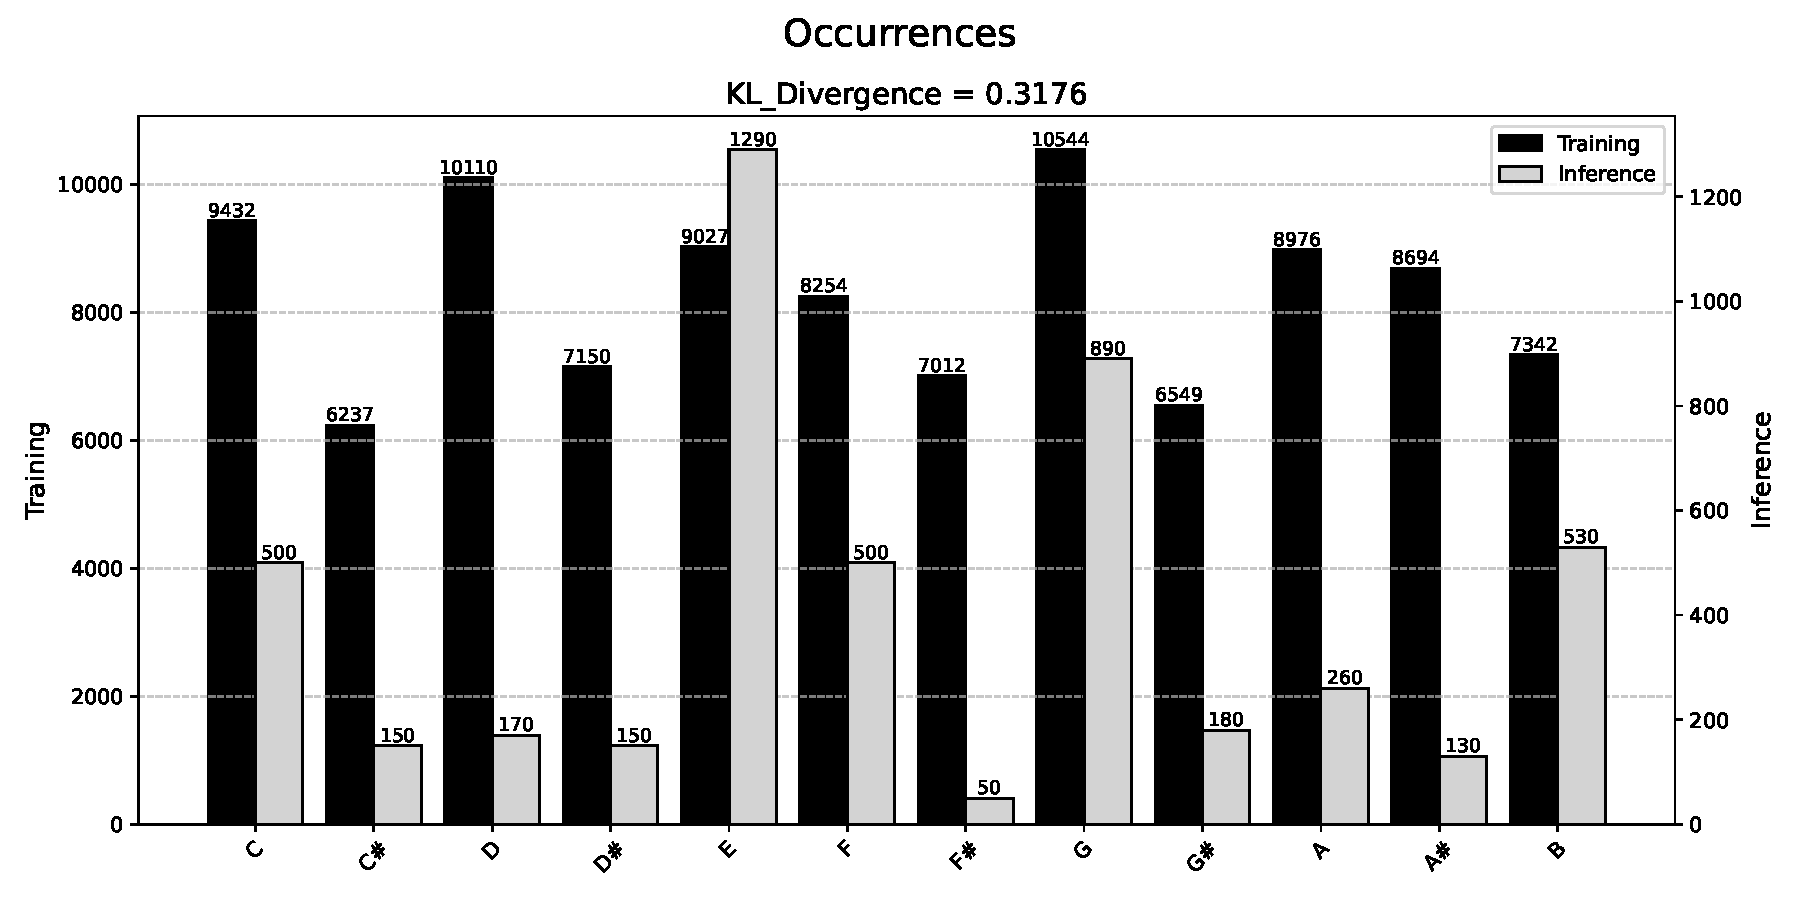
\includegraphics[clip, width=0.9\linewidth]{compareprobabilitynotes.pdf}
\caption{Note occurrences of training data and test data}
  \label{fig:note}
\end{figure}


The model produces musically pleasing sequences, effectively 
combining notes, beats, and accents while maintaining sequence 
context between measures. Evaluation was performed using a temperature setting of 0.7.
\begin{figure}[H]
  \centering

\includegraphics[trim={20 120 0 120}, clip, width=0.8\linewidth]{test_all.pdf}
\caption{Test results showing 5 musical measures}
  \label{fig:inference}
\end{figure}

Implementation details and hyper-parameter settings are provided in the associated GitHub repository \cite{SC0RE}.
% Acknowledgements and Disclosure of Funding should go at the end, before appendices and references

\acks{This research received no specific grant from any funding agency in the public, commercial, or not-for-profit sectors.}

% Manual newpage inserted to improve layout of sample file - not
% needed in general before appendices/bibliography.

\newpage

\appendix
\section{}
\label{app:A}

% Note: in this sample, the section number is hard-coded in. Following
% proper LaTeX conventions, it should properly be coded as a reference:

%In this appendix we prove the following theorem from
%Section~\ref{sec:textree-generalization}:

In this appendix a comprehensive list of accents played on the guitar is provided.

\noindent
\begin{table}[h!]
\centering
\begin{tabular}{|c|c|c|}
\hline
\textbf{Accent} & \textbf{Unique Index} \\
\hline
BAR  & 27049\\
BOS  & 27050\\
BARRE\_NOTE & 27051\\
BEND\_NOTE\_1 & 27052\\
BEND\_NOTE\_2 & 27053\\
BEND\_NOTE\_3 & 27054\\
BEND\_NOTE\_4 & 27055\\
BEND\_NOTE\_5 & 27056\\
BEND\_NOTE\_6 & 27057\\
BEND\_NOTE\_7 & 27058\\
TREM\_BAR\_1 & 27059\\
TREM\_BAR\_2 & 27060\\
TREM\_BAR\_3 & 27061\\
TREM\_BAR\_4 & 27062\\
TREM\_BAR\_5 & 27063\\
DEAD\_NOTE & 27064\\
SLIDE\_NOTE\_1 & 27065\\
SLIDE\_NOTE\_2 & 27066\\
SLIDE\_NOTE\_3 & 27068\\
SLIDE\_NOTE\_4 & 27069\\
SLIDE\_NOTE\_5 & 27070\\
SLIDE\_NOTE\_6 & 27071\\
HAMMER & 27072\\
VIBRATO & 27073\\
HARMONIC\_1 & 27074\\
EOS  & 27075\\
\hline
\end{tabular}
\caption{Example of unique indexing of guitar accents.}
\label{tab:accent_indexing}
\end{table}

\section{}
\label{app:B}
This appendix explains relevant statistics about the dataset used for training and evaluation.
The rhythm guitar tracks were obtained from \cite{SCORESET}.
The dataset consists files in .gp5 format in standard tuning. 
From the full set, a total of 6208 sequences were selected via random sampling for training.
An 80/20 split was used to create the training and validation sets. 
For testing, top 10 first notes of each measure were selected as 
prompts for sequence generation and evaluation.

\section{}
\label{app:C}
In this appendix a comprehensive list of rhythmic patterns are listed.
\noindent
\begin{table}[H]
\centering
\begin{tabular}{|c|c|c|}
\hline
\textbf{Pattern} & \textbf{Unique Index} \\
\hline
Base  & 1 \\
Triplet & 2 \\
Quintuplet & 3 \\
sextuplet & 4 \\
septuplet  & 5 \\
9 tuplets & 6 \\
11-tuplets & 7 \\
Dotted - Base  & 8 \\
Dotted - Triplet & 9 \\
Dotted - Quintuplet & 10 \\
Dotted - sextuplet & 11 \\
Dotted - septuplet  & 12 \\
Dotted - 9 tuplets & 13 \\
Dotted - 11-tuplets & 14 \\
\hline
\end{tabular}
\caption{Example of unique indexing of rhythm.}
\label{tab:rhythmic_indexing}
\end{table}

\section{}
\label{app:D}
This appendix lists hyper-parameter configuration used to generate results.
\begin{table}[h!]
\centering
\begin{tabular}{|c|c|c|}
\hline
\textbf{Property} & \textbf{Value} \\
\hline
FFN\_HIDDEN  & 512 \\
MAX\_SEQ\_LENGTH & 16 \\
NUM\_HEADS & 4 \\
DROP\_PROB & 0.3 \\
NUM\_LAYERS  & 3 \\
D\_MODEL & 512 \\
LEARNING\_RATE & 0.0001 \\
TEMPERATURE  & 1.0 \\
OVERLAP & 8 \\
LAMBDA & 0.5 \\
ALPHA & 0.1 \\
DELTA  & 0.001 \\
\hline
\end{tabular}
\caption{Hyper-parameter values for training.}
\label{tab:hyperparams}
\end{table}

\vskip .2in
\bibliography{TransformerRiffage}

\end{document}
